% =============================================================
%  Estrutura do relatório SAHC, Milestone 2
%  Esqueleto de secções, conteúdo a preencher
% =============================================================

% -------------------------------------------------------------
\section*{Glossário}
\addcontentsline{toc}{section}{Glossário}

\noindent\textbf{DCAP (Data Center Attestation Primitives):} stack da Intel para verificação local de quotes SGX em datacenter, sem dependência em tempo real de servidores Intel.

\noindent\textbf{EPC (Enclave Page Cache):} região de memória física cifrada e autenticada pelo processador onde residem o código e os dados do enclave.

\noindent\textbf{Gramine LibOS:} library OS que permite executar binários Linux não modificados dentro de enclaves SGX, mediante um manifest que declara recursos e políticas.

\noindent\textbf{k-anonymity:} propriedade segundo a qual qualquer resultado divulgado agrega registos de pelo menos $k$ indivíduos distintos, prevenindo reidentificação trivial. Este trabalho aplica $k=5$.

\noindent\textbf{MRENCLAVE:} hash de medição que identifica de forma única o código e a configuração inicial de um enclave, verificado pelo cliente durante a atestação remota.

\noindent\textbf{MRSIGNER:} hash da chave pública do signatário do enclave, identificando a entidade que assinou o binário independentemente da versão.

\noindent\textbf{PCCS (Provisioning Certificate Caching Service):} serviço local que armazena certificados Intel necessários à verificação DCAP.

\noindent\textbf{PCK (Provisioning Certification Key):} chave única do processador, usada pelo Quoting Enclave para assinar quotes que comprovam a autenticidade do hardware.

\noindent\textbf{Quorum:} regra de admissão segundo a qual uma nova identidade só passa a ser reconhecida após reunir um número mínimo de assinaturas de identidades já confiáveis.

\noindent\textbf{Quote:} estrutura assinada produzida pelo Quoting Enclave que veicula a medição do enclave, atributos da plataforma e dados aplicacionais arbitrários, servindo de prova verificável remotamente.

\noindent\textbf{QE (Quoting Enclave):} enclave arquitetural da Intel que assina quotes com a chave de atestação derivada da PCK.

\noindent\textbf{Sealing:} cifra de dados pelo enclave com uma chave derivada da própria identidade, permitindo persistir estado entre execuções sem o expor ao operador da máquina.

\noindent\textbf{SGX (Software Guard Extensions):} extensão do conjunto de instruções x86 da Intel que permite criar enclaves de memória isolados ao nível do processador.

\noindent\textbf{TCB (Trusted Computing Base):} conjunto mínimo de componentes de hardware e software em que o sistema deposita confiança para ser seguro.

% -------------------------------------------------------------
\section{Introdução}

\subsection{Motivação}

A análise colaborativa de dados clínicos entre hospitais, institutos de investigação e autoridades de saúde pública oferece ganhos relevantes em deteção precoce de surtos, avaliação de eficácia terapêutica e investigação biomédica em geral. Os mesmos dados que tornam estas análises valiosas são, no entanto, registos pessoais sensíveis cuja exposição configura violações regulatórias graves ao abrigo do RGPD e da HIPAA, com consequências severas para os titulares.

As proteções clássicas, nomeadamente cifra em repouso, controlo de acesso baseado em roles e auditoria, são necessárias mas insuficientes. O ponto fraco continua a ser o momento da computação, em que os dados têm de ser desencriptados para que o motor de queries os possa processar e ficam expostos ao sistema operativo, ao hypervisor e, em ambiente cloud, ao próprio operador da infraestrutura. Um adversário com acesso privilegiado ao sistema contorna todos os controlos lógicos e lê a memória do processo em execução.

Os Trusted Execution Environments respondem a este problema deslocando a confiança para uma fronteira garantida por hardware. Ao isolar a execução de código sensível em enclaves protegidos pelo processador, garantem confidencialidade e integridade do que lá dentro corre mesmo perante um sistema operativo ou um hypervisor maliciosos. O Intel SGX é a tecnologia escolhida neste trabalho por oferecer uma combinação madura de atestação remota, isolamento ao nível da página e ecossistema de ferramentas, viável em hardware comercial de datacenter.

O cenário concreto considerado é um consórcio de hospitais que acordam contribuir registos para um data lake confidencial alojado em cloud não confiável, sobre o qual investigadores autorizados emitem queries agregadas. O sistema deve garantir que o operador cloud nunca tem acesso a registos individuais, que cada participante pode verificar criptograficamente que o código em execução é o pretendido, e que apenas resultados agregados acima de um limiar mínimo de registos saem do enclave.

\subsection{Da Milestone 1 à Milestone 2}

A Milestone 1 entregou um protótipo monolítico em modo de simulação que validou o fluxo end-to-end fundamental (atestação simulada, AES-128-GCM, upload e queries agregadas em memória) num único processo e sem verificação real de cadeia de certificados Intel. As funcionalidades de identidade, sealing, k-anonymity e motor SQL real ficaram para a Milestone 2.

A Milestone 2 fecha essa lista. O sistema passa a ter dois binários, sgx\_server e sgx\_client sobre TCP, com handshake que combina atestação, ECDH P-256 e binding criptográfico do nonce ao quote, derivação HKDF-SHA256 e canal AEAD com sequence numbers. Cada participante tem uma identidade ECDSA P-256 long-term e recebe role na admissão; hospitais entram como founders, investigadores entram por quorum de assinaturas de hospitais. O enclave aplica role enforcement e k-anonymity com $k=5$ em todos os resultados, e persiste estado em disco via sealing MRENCLAVE-bound. O target de produção é o caminho Gramine sobre hardware Intel SGX com DCAP real e DuckDB embutido como motor SQL; o caminho SGX SDK em SIM mantém-se na codebase apenas como ambiente de desenvolvimento e validação local. Os dois caminhos partilham um trusted core neutro de backend, escrito em C, que isola sessões, identidades, k-anonymity e crypto aplicacional da escolha de runtime. Toda esta camada foi validada em hardware Intel SGX numa máquina Azure DCsv3.

% -------------------------------------------------------------
\section{Contexto e Fundamentos Técnicos}

% Material já apresentado em maior detalhe na Milestone 1; aqui reduzido aos elementos diretamente mobilizados pelo M2.

\subsection{Intel SGX e atestação remota DCAP}

O Intel SGX~\cite{costan2016sgx,anati2013innovative} é a tecnologia central deste trabalho. O modelo de confiança coloca apenas o processador na TCB do enclave, considerando hostis o sistema operativo, o hypervisor e o restante software da máquina. A proteção assenta no Enclave Page Cache, região de memória física cifrada e autenticada pelo processador. Cada enclave tem uma identidade criptográfica única, o MRENCLAVE, derivada do hash do código carregado no arranque, e é este o valor verificado pelo cliente durante a atestação remota.

A atestação permite a uma entidade externa confirmar que comunica com um enclave legítimo, executando código não modificado, num processador Intel genuíno. O modelo clássico EPID dependia de servidores Intel centralizados; o DCAP, adoptado neste trabalho~\cite{intel2018dcap}, desloca a verificação para o próprio datacenter. O Quoting Enclave assina o report local com uma chave ECDSA derivada da PCK do processador, produzindo um quote, e o verificador encadeia essa assinatura até à raiz Intel a partir de certificados obtidos via PCCS. O resultado é uma cadeia de evidência verificável offline, com o operador do datacenter a oferecer atestação completa sem conectividade em tempo real com a Intel.

\subsection{Gramine LibOS}

O Gramine LibOS~\cite{tsai2017graphene,gramine_project} é o runtime adoptado para execução em hardware. É uma library OS que emula a interface POSIX dentro do enclave, permitindo correr binários Linux não modificados, com syscalls servidas internamente quando possível ou exportadas sob fronteira controlada quando inevitáveis. A configuração é feita por um manifest declarativo que enumera recursos e, criticamente, os ficheiros que entram na medição do MRENCLAVE. A vantagem prática para este projeto é tornar viável a integração de um motor SQL completo (DuckDB~\cite{raasveldt2019duckdb}) dentro do enclave sem reescrever as suas chamadas ao sistema. O custo é uma TCB significativamente maior, com o LibOS, as suas dependências e o motor SQL a passarem todos a integrar o código medido.

\subsection{Estado da arte}

A investigação em analytics confidencial sobre SGX produziu várias contribuições relevantes. Opaque~\cite{zheng2017opaque} integra Spark com SGX e oculta padrões de acesso; EnclaveDB~\cite{priebe2018enclavedb} aloja uma base de dados relacional dentro do enclave com proteção contra rollback; VC3~\cite{schuster2015vc3} focou-se em jobs MapReduce confidenciais. O caminho Gramine+DuckDB deste projeto apoia-se directamente nestas contribuições. No domínio da saúde, EHDEN~\cite{ehden} demonstrou análises federadas sobre OMOP CDM partilhando apenas agregados; SMPC dá garantias formais de privacidade ao custo de overhead proibitivo para queries complexas; a combinação de TEEs com privacidade diferencial~\cite{dwork2006differential} aparece em trabalhos recentes como extensão natural prioritária. Em hardware concorrente, AMD SEV~\cite{kaplan2016sev} opera ao nível de VM com TCB mais extensa, ARM TrustZone é mais adequado a DRM, e RISC-V Keystone~\cite{lee2020keystone} carece de ecossistema maduro. SGX mantém o melhor equilíbrio entre maturidade, expressividade e desempenho para o cenário considerado.

% -------------------------------------------------------------
\section{Modelo de Sistema e Adversário}

\subsection{Entidades e papéis}

O sistema opera num cenário com quatro classes de entidades. Os hospitais são as fontes primárias de dados, contribuindo registos clínicos previamente cifrados para o data lake. Os investigadores são consumidores que emitem queries agregadas sobre o conjunto de dados combinado, sem nunca observar registos individuais. O operador cloud aloja a infraestrutura física e o sistema operativo da máquina onde o servidor corre, mas não é considerado confiável. O administrador do consórcio é responsável por curar a lista de identidades autorizadas, definindo founders e validando approvals que entram no ficheiro \texttt{authorized\_parties.json}.

Cada hospital ou investigador é uma identidade autenticada por um par de chaves ECDSA P-256 long-term, gerado localmente e cuja chave pública é registada no ficheiro de identidades autorizadas. As capacidades atribuídas a cada role estão sumarizadas na Tabela~\ref{tab:roles}.

\begin{table}[H]
\centering
\begin{tabular}{lccc}
\toprule
Role & Upload & Query & Limiar k-anonymity \\
\midrule
Hospital & sim & sim & 5 \\
Researcher & não & sim & 5 \\
\bottomrule
\end{tabular}
\caption{Capacidades por role.}
\label{tab:roles}
\end{table}

A admissão de novas identidades segue dois caminhos. Os hospitais entram no sistema como founders, sendo registados diretamente pelo administrador na lista autorizada. Os investigadores são admitidos por quorum, o que significa que a sua entrada só é aceite pelo enclave depois de reunir pelo menos $M$ assinaturas válidas de hospitais já reconhecidos sobre uma representação canónica da identidade do investigador. Este trabalho usa $M=2$ por configuração padrão. O quorum desloca a decisão de admissão para o conjunto de participantes, evitando que um único administrador possa adicionar identidades arbitrárias sem o conhecimento do consórcio.

\subsection{Modelo de adversário}

O adversário considerado tem capacidades de operador cloud com acesso privilegiado ao sistema operativo, ao hypervisor e ao hardware da máquina que aloja o servidor, à exceção do interior do enclave. Pode ler e modificar livremente memória convencional do processo, ler e modificar tráfego de rede, observar e manipular o sistema de ficheiros, e reiniciar o servidor a qualquer momento. Pode ainda colaborar com partes externas que se identifiquem como hospitais ou investigadores, na tentativa de obter dados em claro, escalar role ou desviar o sistema do seu comportamento previsto.

Os parágrafos seguintes estruturam o modelo em duas vistas. A primeira enumera as classes de ataque que estão dentro do escopo e identifica, para cada uma, o mecanismo concreto que o sistema usa para a mitigar. A segunda enumera classes que estão fora do escopo e justifica, para cada uma, a razão da exclusão.

\paragraph{Ataques considerados.}

\begin{description}
  \item[A1, leitura de memória do processo servidor.] Um operador com privilégios de root no host pode invocar \texttt{ptrace}, ler \texttt{/proc/<pid>/mem} ou anexar um debugger.

  \textbf{Mitigação.} Os registos clínicos e as chaves de sessão residem exclusivamente em páginas EPC, cifradas e autenticadas pelo processador. Qualquer leitura fora do enclave devolve apenas ciphertext sem utilidade.
  \item[A2, manipulação de tráfego de rede.] Um adversário em posição de man-in-the-middle pode intercetar, modificar, reordenar ou repetir mensagens entre cliente e servidor.

  \textbf{Mitigação.} Canal AEAD com AES-128-GCM, sequence numbers monotónicos por sentido e tipo da mensagem coberto pela AAD, descritos na secção~5.3.
  \item[A3, impersonação de enclave.] Um adversário pode tentar substituir o enclave legítimo por código arbitrário em user-space, ou fazer downgrade de uma execução em hardware para simulação.

  \textbf{Mitigação.} Atestação remota com quote DCAP no caminho HW, MRENCLAVE pinned a partir do binário assinado, recusa explícita de quotes SAHC quando o cliente exige DCAP (secção~6.4).
  \item[A4, replay ou substituição do quote.] O adversário pode tentar reutilizar um quote produzido para uma sessão anterior, ou intercalar a sua própria chave pública efémera no \texttt{ATTEST\_RESP}.

  \textbf{Mitigação.} O \texttt{report\_data} do quote carrega \texttt{SHA-256(nonce $\|$ enclave\_ecdh\_pub)}, o que vincula o quote ao nonce escolhido pelo cliente e à chave efémera do enclave, descrito na secção~5.2.
  \item[A5, impersonação de cliente.] Um adversário pode tentar abrir sessão fingindo ser um hospital ou investigador legítimo, ou submeter mensagens em nome de uma identidade que não controla.

  \textbf{Mitigação.} Cada cliente assina, com a sua chave long-term ECDSA P-256, uma representação canónica que liga o domínio (\texttt{SAHC-attest-v1}), o nonce e a chave pública efémera, verificada pelo enclave antes da admissão.
  \item[A6, escalada de role.] Um cliente investigador admitido pode tentar emitir uma mensagem \texttt{MSG\_UPLOAD}, restrita ao role hospital.

  \textbf{Mitigação.} O role é fixado no \texttt{KEY\_ACK} a partir do ficheiro de identidades autorizadas, e o trusted core verifica-o antes de qualquer decifragem aplicacional, devolvendo \texttt{E\_UNAUTHORIZED} sem inspecionar o conteúdo (secção~5.4).
  \item[A7, admissão de identidade não autorizada.] O adversário pode tentar inserir uma chave pública adversarial no ficheiro de identidades autorizadas, ou forjar uma approval de hospital.

  \textbf{Mitigação.} Quorum de $M=2$ assinaturas válidas de hospitais já reconhecidos sobre uma representação canónica do investigador, com prefixo de domínio distinto do handshake, validado pelo enclave no carregamento (secção~4.3).
  \item[A8, inferência por agregados.] Um cliente legítimo pode emitir queries cujo conjunto correspondente é tão pequeno que o agregado revela um indivíduo.

  \textbf{Mitigação.} Limiar de k-anonymity com $k=5$ aplicado no trusted core, com fail-closed sem exposição parcial do agregado quando o limiar não é satisfeito (secção~7.5).
  \item[A9, leitura ou troca do estado persistido.] O adversário pode copiar o blob sealed e tentar desselá-lo numa máquina diferente, ou substituí-lo pelo blob de um enclave alternativo.

  \textbf{Mitigação.} Sealing com key policy MRENCLAVE-bound, o que vincula a chave de unsealing à medição exata do enclave em execução e à plataforma física, satisfazendo RS9 (secção~7.4).
\end{description}

\paragraph{Ataques fora do escopo.}

\begin{description}
  \item[O1, canais laterais sobre o enclave.] Ataques por timing, cache ou page-fault contra o código do enclave estão fora do escopo. O sistema adopta padrões de tempo constante em pontos críticos (comparação de MAC), mas não foi sujeito a verificação exaustiva nem a mitigações dedicadas como Aex-notify ou scheduling consciente de hyperthreading. Listado como trabalho futuro em~9.3.
  \item[O2, ataques físicos ao processador.] Modificação de hardware, sondas em barramentos, fault injection e ataques eletromagnéticos exigem acesso físico que não corresponde ao adversário cloud considerado, e são endereçados pelos modelos formais da própria Intel.
  \item[O3, comprometimento de endpoints legítimos.] Se a chave long-term de um hospital ou investigador for exfiltrada da máquina do utilizador, o adversário herda o role correspondente. A custódia das chaves nos endpoints é responsabilidade dos participantes e está fora do alcance do enclave.
  \item[O4, negação de serviço.] O protótipo não tem rate limiting nem proteção contra flooding de \texttt{ATTEST\_REQ}. Um adversário com largura de banda suficiente pode esgotar o pool de oito sessões. Considerado fora do escopo dado que DoS não compromete confidencialidade ou integridade, apenas disponibilidade, e a mitigação habitual (load balancer, firewall) vive fora da fronteira do enclave.
  \item[O5, revogação dinâmica.] A revogação de uma identidade exige re-curação manual do ficheiro de identidades autorizadas e reinício do servidor. A revogação online não está implementada e está listada como trabalho futuro.
  \item[O6, bugs no código.] O trusted core não é formalmente verificado. Vulnerabilidades de memória ou erros lógicos no enclave podem comprometer todas as outras propriedades. Mitigado por uma TCB pequena (caminho SDK) e por backends intercambiáveis que reduzem a duplicação, mas não eliminado.
  \item[O7, rollback do estado persistido.] Um adversário com acesso ao sistema de ficheiros pode repor um blob sealed antigo, fazendo o enclave regredir a um estado anterior. O sistema atual não tem contador monotónico que detete a regressão. Listado como prioridade alta em~9.3.
\end{description}

A separação explícita entre as classes A e O define a fronteira do que este protótipo se propõe a garantir. Tudo o que cai em A é tratado por construção; tudo o que cai em O é honestamente reportado como limitação, com remissão para o trabalho futuro quando aplicável.

\subsection{Requisitos funcionais}

\begin{description}
  \item[RF1, ingestão cifrada.] Um cliente com role Hospital pode submeter um conjunto de registos clínicos cifrados com a chave de sessão estabelecida, e o servidor confirma o número de registos aceites.
  \item[RF2, queries agregadas.] Um cliente com role Hospital ou Researcher pode emitir uma query agregada sobre o conjunto unificado de registos e receber o valor agregado, o número de registos correspondentes e o limiar $k$ aplicado.
  \item[RF3, agregações suportadas.] O sistema suporta as operações AVG, MIN, MAX e COUNT no caminho SGX SDK, e SQL agregado restrito a uma allowlist no caminho Gramine com DuckDB embutido.
  \item[RF4, multi-sessão concorrente.] O servidor mantém sessões independentes para múltiplos clientes em simultâneo, com isolamento entre estados de sessão.
  \item[RF5, persistência transparente.] O estado do enclave, identidades reconhecidas e registos ingeridos sobrevive a um reinício do servidor sem requerer re-upload por parte dos hospitais.
  \item[RF6, identidade reproduzível.] Cada participante pode gerar a sua identidade ECDSA localmente e fornecê-la ao consórcio, com o sistema a aceitá-la apenas se passar pelo processo de admissão definido na secção 3.1.
\end{description}

\subsection{Requisitos de segurança}

\begin{description}
  \item[RS1, confidencialidade dos registos.] Os registos clínicos individuais nunca são observáveis em claro fora do enclave, em qualquer ponto da pipeline, mesmo perante um operador cloud com acesso total à máquina.
  \item[RS2, integridade dos registos e dos resultados.] Qualquer modificação a registos cifrados em trânsito, ou a resultados de query devolvidos pelo enclave, é detetada e rejeitada pelo recetor.
  \item[RS3, autenticidade do enclave.] O cliente verifica criptograficamente, antes de partilhar qualquer dado, que está a comunicar com um enclave que executa o código pretendido num processador Intel genuíno.
  \item[RS4, autenticidade dos clientes.] O enclave verifica criptograficamente a identidade long-term de cada cliente antes de derivar uma chave de sessão.
  \item[RS5, resistência a replay.] O canal seguro deteta replays de frames através de sequence numbers monotónicos por sentido, e o handshake é protegido por nonces frescos com binding ao quote.
  \item[RS6, role enforcement.] O enclave rejeita qualquer mensagem aplicacional cujo tipo não seja permitido para o role atribuído à sessão.
  \item[RS7, admissão controlada.] Nenhuma identidade de investigador é aceite sem reunir o quorum mínimo de assinaturas de hospitais sobre a sua representação canónica, validado pelo enclave no carregamento do estado.
  \item[RS8, forward secrecy parcial.] Cada sessão deriva chaves a partir de um par ECDH efémero do enclave, pelo que o comprometimento futuro do material de longo prazo do enclave não permite decifrar tráfego capturado de sessões já encerradas.
  \item[RS9, sealing vinculado à identidade do enclave.] O estado persistido em disco só pode ser desselado por um enclave com o mesmo MRENCLAVE, garantindo que um operador malicioso não consegue desviar registos para um enclave alternativo.
  \item[RS10, k-anonymity nos resultados.] Nenhum resultado de query é devolvido se agregar menos de $k$ registos, com $k=5$ no protótipo.
\end{description}

% -------------------------------------------------------------
\section{Arquitetura do Sistema}

\subsection{Visão split-trust e separação cliente-servidor}

A arquitetura adotada é uma evolução direta do modelo split-trust do Intel SGX, em que cada elemento computacional é classificado como confiável ou não confiável e a fronteira entre os dois é fixada em hardware. O lado não confiável compreende o sistema operativo da máquina cloud, o processo servidor que gere a rede e os ficheiros, e qualquer biblioteca convencional aí carregada. O lado confiável corresponde ao código que corre dentro do enclave, à memória EPC que o aloja e às chaves derivadas pelo processador para esse enclave.

A Milestone 2 quebra a unidade de processo do protótipo anterior em duas aplicações separadas. O \texttt{sgx\_server} é o processo persistente que aloja o enclave, escuta numa porta TCP e dispatcha conexões para slots de sessão geridos pelo trusted core. O \texttt{sgx\_client} é uma aplicação leve que cada participante corre na sua própria máquina, executa o handshake de atestação e canal seguro, e expõe um REPL ou um modo single-shot para emitir mensagens aplicacionais. Esta separação tem três consequências práticas. Primeiro, formaliza um adversário de rede com capacidade de manipular tráfego entre cliente e servidor, alinhando o protótipo com o cenário cloud realista. Segundo, permite que múltiplos clientes coexistam sobre um mesmo servidor, com sessões concorrentes isoladas. Terceiro, reduz a TCB do cliente ao mínimo, dado que o cliente não aloja qualquer enclave e só precisa de bibliotecas criptográficas user-space para participar.

A comunicação entre cliente e servidor usa sockets TCP em texto binário, com framing aplicacional próprio descrito na secção~5. A escolha de não usar TLS é deliberada. A atestação remota do enclave já fornece autenticação do servidor com uma propriedade mais forte do que a que TLS oferece, dado que vincula o tráfego a um conjunto específico de bytes de código verificado pelo cliente. A identidade long-term do cliente é por sua vez autenticada por assinatura ECDSA aplicada na primeira mensagem do handshake, autenticando o cliente com a granularidade de role e quorum exigida pelo modelo de adversário, granularidade que TLS por si só não captura.

\subsection{Trusted core neutro de backend}

O coração do servidor é um trusted core escrito em C, fisicamente concentrado no diretório \texttt{EnclaveLogic/}, que implementa toda a lógica de negócio sensível. Inclui a gestão de slots de sessão, o carregamento e validação do ficheiro de identidades autorizadas com verificação de quorum, o handshake combinado de atestação e ECDH, a derivação de chaves, a aplicação do canal seguro, o role enforcement nas mensagens aplicacionais, a aplicação do limiar k-anonymity, o sealing do estado e a sua recuperação no arranque. Este módulo é deliberadamente agnóstico em relação ao runtime de enclave que o aloja.

A neutralidade é obtida através de um padrão de backend interfaces. Para cada serviço dependente da plataforma o trusted core declara uma API minimalista num cabeçalho, e existem duas implementações intercambiáveis dessa API. O backend de criptografia simétrica e ECDH, declarado em \texttt{crypto\_backend.h}, tem uma realização em SGX tcrypto para o caminho SDK e uma realização em OpenSSL para o caminho Gramine. O backend de identidade, declarado em \texttt{identity\_backend.h}, encapsula a verificação de assinaturas ECDSA dos clientes e do quorum dos hospitais. O backend de sealing, em \texttt{seal\_backend.h}, abstrai a obtenção da sealing key e a cifra ou desencriptação do blob persistente. O motor de queries, declarado em \texttt{query\_engine.h}, tem duas implementações independentes, um motor artesanal que percorre o array em memória e calcula AVG, MIN, MAX e COUNT, e um motor sobre DuckDB embutido que avalia SQL agregado restrito a uma allowlist.

A consequência prática deste desenho é que migrar entre runtimes não toca na lógica de negócio. O Makefile compila duas variantes de cada ficheiro do trusted core, uma para cada caminho, escolhendo o backend apropriado em cada compilação. O ficheiro de fronteira do SGX SDK reduz-se a uma camada fina sobre as ECALLs que reencaminha argumentos para funções do trusted core, e o ponto de entrada do servidor Gramine invoca o mesmo trusted core diretamente sem passar por uma fronteira de ECALLs. A reutilização efetiva é elevada e foi um requisito importante para conseguir cumprir as fases 3 e 4 dentro do orçamento de tempo do projeto.

\subsection{Modelo de identidades com admissão por quorum}

Cada participante é representado por um par de chaves ECDSA P-256 long-term gerado localmente através de um script de utilidade. A chave pública é entregue ao administrador do consórcio, que a regista no ficheiro \texttt{authorized\_parties.json} associada a um identificador legível e a um role. O ficheiro tem três campos relevantes, a versão do esquema, o parâmetro $M$ do quorum, e duas listas que enumeram hospitais e investigadores autorizados.

Os hospitais são founders por construção e a sua presença no ficheiro é suficiente para serem aceites pelo enclave. Os investigadores requerem uma lista adicional de approvals, em que cada entrada associa um identificador de hospital e a sua assinatura ECDSA sobre uma representação canónica do investigador. A representação canónica é construída como o digest SHA-256 da concatenação de uma string de domínio fixa, do identificador do investigador e da chave pública do investigador. A string de domínio impede que assinaturas produzidas para outro propósito possam ser reaproveitadas como approvals.

O enclave valida o ficheiro durante o arranque, dentro da memória protegida. Para cada investigador, conta as approvals cujas assinaturas verificam contra chaves de hospitais já reconhecidos e descarta a entrada se o número for inferior a $M$. O parâmetro $M$ é configurável e este trabalho usa $M=2$ como padrão, suficiente para tornar a admissão dependente de pelo menos dois hospitais distintos. Identidades que falhem a verificação são silenciosamente ignoradas em vez de causarem abort, o que permite que uma versão adiantada do ficheiro contendo entradas ainda incompletas seja distribuída sem partir o servidor.

\subsection{Visão global em diagrama}

A Figura~\ref{fig:arch} sintetiza os elementos descritos nas subsecções anteriores.

\begin{figure}[H]
  \centering
  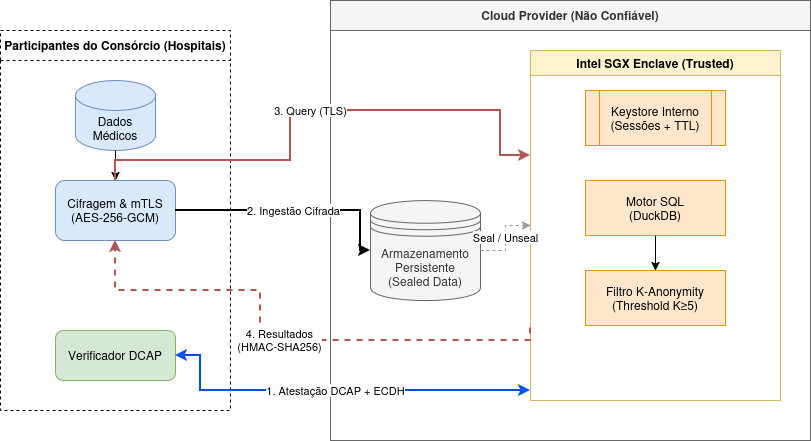
\includegraphics[width=0.95\textwidth]{pictures/architecture}
  \caption{Arquitetura global do sistema com fronteira de confiança e backends intercambiáveis.}
  \label{fig:arch}
\end{figure}

% -------------------------------------------------------------
\section{Protocolo Seguro}

\subsection{Wire protocol e framing}

A comunicação entre cliente e servidor decorre sobre uma única ligação TCP por sessão e usa um canal seguro próprio, em vez de TLS. A escolha não decorre de uma preferência por minimalismo mas da observação de que TLS standard não oferece a propriedade central que o sistema exige, a saber, o binding criptográfico entre a chave de sessão e o código medido do enclave. Sem esse binding, um adversário com acesso ao host não confiável pode terminar TLS fora do enclave e observar o tráfego em claro, dado que TLS autentica o servidor com base num certificado X.509 cuja chave privada vive em memória convencional. A variante RA-TLS, que injeta a evidence de atestação em extensões X.509 e desloca a verificação para o cliente, fecha esse buraco mas implica importar uma stack TLS completa para dentro da TCB e escrever a verificação custom das extensões na mesma, sem ganho líquido em superfície de auditoria. A construção adoptada estabelece o binding diretamente no \texttt{report\_data} do quote, descrito na secção~5.2, e mantém o canal cifrado restrito a uma camada AEAD fina por cima de TCP, com o efeito secundário, e não objetivo, de simplificar a auditoria. Cada frame da camada de rede tem o formato \texttt{type(1) | len(4 BE) | payload(len)}, com o byte de tipo a identificar a mensagem aplicacional, o comprimento em big-endian e o payload em bruto. O parser do recetor enforça um teto absoluto de \texttt{FRAME\_MAX\_PAYLOAD} bytes, fixado em 16 MiB, antes mesmo de qualquer alocação, fechando a porta a ataques de exaustão de memória por campo de comprimento adversarial.

O conjunto de tipos aplicacionais é fechado e enumerado em \texttt{Include/protocol.h}. Os tipos pré-KEX, a saber \texttt{MSG\_ATTEST\_REQ} e \texttt{MSG\_ATTEST\_RESP}, transportam payload em claro porque ainda não existe chave de sessão estabelecida e a sua autenticidade é garantida por outras vias, designadamente a assinatura ECDSA do cliente e a assinatura do quote pelo Quoting Enclave. Os tipos pós-KEX, que incluem \texttt{MSG\_KEY\_CONFIRM}, \texttt{MSG\_UPLOAD}, \texttt{MSG\_QUERY\_REQ} e respetivos acks, transportam um envelope cifrado com o seguinte layout interno, descrito no cabeçalho \texttt{secure\_frame.h},

\begin{center}
\texttt{seq(8 BE) | iv(12) | ciphertext(N) | tag(16)}
\end{center}

\noindent em que o IV é composto por um prefixo de 4 bytes derivado por HKDF e pelos 8 bytes do número de sequência, e o tag é o tag de autenticação AES-GCM de 16 bytes. A AAD coberta pela cifra é a concatenação \texttt{type(1) || seq(8 BE)} de 9 bytes, escolhida deliberadamente para vincular cada criptograma ao seu tipo aplicacional e à sua posição na sequência da sessão. O overhead total por frame pós-KEX fixa-se em 36 bytes acima do plaintext, o que é amortizado de forma natural pelo upload de blocos de registos e por respostas de query agregadas.

\subsection{Handshake combinado}

O handshake da Milestone 2 combina três objetivos numa só troca de mensagens, atestação remota do enclave, autenticação da identidade long-term do cliente e estabelecimento de uma chave de sessão por ECDH efémero. A combinação é deliberada e tem como propriedade central o binding criptográfico do nonce do cliente à chave pública efémera do enclave, descrito mais à frente.

A primeira mensagem é \texttt{MSG\_ATTEST\_REQ}, enviada pelo cliente. O payload contém o identificador da party, um nonce fresco de 16 bytes, a chave pública ECDH P-256 do cliente em formato uncompressed e uma assinatura ECDSA P-256 produzida com a chave long-term do cliente sobre a representação canónica

\begin{center}
\texttt{"SAHC-attest-v1" || nonce || client\_ecdh\_pub}
\end{center}

\noindent A string de domínio \texttt{SAHC-attest-v1} impede que assinaturas geradas para outras estruturas, em particular as approvals do quorum, possam ser reaproveitadas como assinaturas de handshake. O servidor consulta a tabela de identidades autorizadas carregada no arranque, valida a assinatura sobre essa representação canónica e rejeita a sessão se a party for desconhecida ou a assinatura não verificar.

Com o cliente autenticado, o enclave gera um par ECDH P-256 efémero, computa o segredo partilhado, deriva a chave de sessão e prepara o quote. O quote (em formato SAHC artesanal no caminho SDK em SIM, em formato DCAP real no caminho Gramine, ver secção 6) carrega no campo \texttt{report\_data} de 32 bytes o valor \texttt{SHA-256(nonce || enclave\_ecdh\_pub)}. Esta construção é o ponto de fecho do handshake, porque vincula simultaneamente ao quote duas grandezas, o nonce escolhido pelo cliente, que prova frescura, e a chave pública efémera do enclave, que prova que quem assinou a chave pertence ao código medido. Um adversário que tente reutilizar um quote anterior falha por não conseguir produzir o mesmo \texttt{report\_data} para um nonce novo, e um adversário que tente intercalar a sua própria chave efémera falha por não conseguir produzir um quote válido sobre um \texttt{report\_data} diferente.

O servidor responde com \texttt{MSG\_ATTEST\_RESP}, cujo primeiro byte indica o formato do quote. O cliente verifica a cadeia de assinaturas (artesanal ou DCAP, conforme a secção 6), recomputa \texttt{SHA-256(nonce || enclave\_ecdh\_pub)} a partir do nonce que enviou e da chave efémera devolvida, e compara o resultado com o \texttt{report\_data} do quote recebido. Em caso de divergência, ou de mismatch contra o \texttt{MRENCLAVE} pinned, a sessão é abortada antes de qualquer dado aplicacional ser enviado.

A terceira e quarta mensagens fecham o handshake. O cliente envia \texttt{MSG\_KEY\_CONFIRM}, contendo \texttt{HMAC-SHA256(session\_key, "confirm")}, prova explícita de que conhece a mesma chave que o enclave derivou. O enclave verifica o MAC em tempo constante e responde com \texttt{MSG\_KEY\_ACK}, que devolve o role atribuído à sessão (hospital ou researcher) consultado a partir da identidade do cliente. A partir deste ponto o canal seguro está estabelecido e todas as mensagens posteriores transitam cifradas. A Figura~\ref{fig:handshake} ilustra o fluxo completo.

\begin{figure}[H]
\centering
\begin{tikzpicture}[font=\footnotesize, >={Stealth[length=2mm]}]
% lifelines
\node[draw, rounded corners, fill=gray!10] (C) at (0,0) {\textbf{Cliente}};
\node[draw, rounded corners, fill=gray!10] (E) at (10,0) {\textbf{Servidor + Enclave + QE}};
\draw[dashed] (0,-0.4)  -- (0,-10.6);
\draw[dashed] (10,-0.4) -- (10,-10.6);

% 1. ATTEST_REQ
\draw[->] (0,-1) -- (10,-1)
  node[midway, above] {\texttt{ATTEST\_REQ} \ party\_id, nonce, ecdh\_pub, sig};

% server-side note
\node[draw, fill=blue!5, align=left, anchor=west, text width=6.2cm]
  at (3.7,-2.4) {verify ECDSA do cliente \\
                 gen ECDH efémero \\
                 report\_data $=$ SHA-256(nonce $\|$ ecdh\_pub) \\
                 produzir quote (SAHC ou DCAP via QE)};

% 2. ATTEST_RESP
\draw[<-] (0,-4.2) -- (10,-4.2)
  node[midway, above] {\texttt{ATTEST\_RESP} \ format, quote, ecdh\_pub};

% client-side note
\node[draw, fill=green!5, align=left, anchor=east, text width=6.2cm]
  at (6.3,-5.5) {verify cadeia (DCAP via QvL ou SAHC) \\
                 recomputar SHA-256, comparar report\_data \\
                 verificar MRENCLAVE pin \\
                 derivar session\_key e iv\_prefix (HKDF)};

% 3. KEY_CONFIRM
\draw[->] (0,-7.3) -- (10,-7.3)
  node[midway, above] {\texttt{KEY\_CONFIRM} \ HMAC(K, ``confirm'')};

% server note
\node[draw, fill=blue!5, align=left, anchor=west, text width=4.5cm]
  at (5.4,-8.4) {verify HMAC em tempo constante \\
                 fixar role da sessão};

% 4. KEY_ACK
\draw[<-] (0,-9.5) -- (10,-9.5)
  node[midway, above] {\texttt{KEY\_ACK} \ status, role};

% bottom marker
\draw[very thick, gray] (0,-10.4) -- (10,-10.4);
\node at (5,-10.1) {\textit{canal AES-128-GCM com sequence numbers estabelecido}};
\end{tikzpicture}
\caption{Handshake combinado de atestação remota e troca de chaves.}
\label{fig:handshake}
\end{figure}

\subsection{Derivação de chaves e canal AEAD}

A derivação de chaves é feita com HKDF-SHA256~\cite{krawczyk2010hkdf} a partir do segredo ECDH partilhado de 32 bytes. O passo de extract usa como salt a string fixa \texttt{SAHC-v1}, gerando um pseudo-random key intermédio. O passo de expand é instanciado duas vezes com infos distintas para produzir material independente, \texttt{"session-aes128"} para a chave AES-128 de 16 bytes do canal seguro e \texttt{"iv-prefix"} para os 4 bytes de prefixo de IV específicos da sessão. A separação de domínios garante que o conhecimento de uma das saídas não revela informação sobre a outra, o que é particularmente relevante porque o IV prefix é tratado como público no envelope e a chave AES é o segredo a proteger.

O canal seguro usa AES-128-GCM como AEAD. O IV de 12 bytes é a concatenação do prefixo de 4 bytes derivado por HKDF e do número de sequência de 8 bytes em big-endian. Esta construção é uma instância do esquema descrito em RFC 5288 para TLS 1.2 e tem a propriedade de tornar a reutilização de nonce estruturalmente impossível desde que o sequence number nunca rebobine, o que num \texttt{uint64\_t} significa nunca em prática. Cada sentido da sessão tem o seu próprio contador, \texttt{seq\_send} e \texttt{seq\_recv}, ambos iniciados a zero e incrementados de uma unidade por mensagem aceite. Um frame com sequence number diferente do esperado é rejeitado pelo recetor sem ser processado, o que detecta tanto reordenação como replay de mensagens dentro da sessão.

A AAD de 9 bytes \texttt{type || seq} cobre as duas grandezas que faltam ao texto cifrado para identificar inequivocamente o frame. O byte de tipo previne ataques de cross-type confusion em que um adversário troca um \texttt{MSG\_UPLOAD\_ACK} por um \texttt{MSG\_QUERY\_RESP}, o sequence number na AAD redunda a proteção do IV mas é o que efetivamente é validado pelo enclave dentro de \texttt{session\_decrypt\_envelope}.

Cada sessão dispõe de chaves derivadas a partir de um par ECDH efémero do enclave, gerado no momento da atestação e descartado após o handshake. Esta escolha confere forward secrecy parcial, no sentido em que o comprometimento futuro do material long-term do enclave (chave de assinatura do quote no caminho SAHC ou PCK no caminho DCAP) não permite recuperar segredos de sessões já encerradas, dado que esse material nunca foi misturado na chave AES.

\subsection{Mensagens aplicacionais}

Estabelecido o canal seguro, o protocolo aceita dois pares de mensagens aplicacionais, um par de upload formado por \texttt{MSG\_UPLOAD} e \texttt{MSG\_UPLOAD\_ACK} e um par de query formado por \texttt{MSG\_QUERY\_REQ} e \texttt{MSG\_QUERY\_RESP}, ambos cifrados pelo envelope descrito na secção~5.1.

O payload em claro do \texttt{MSG\_UPLOAD} é uma sequência contígua de \texttt{PatientRecord} no formato definido em \texttt{Include/types.h}, precedida de um cabeçalho com o número de registos. O enclave decifra o envelope, valida o role da sessão contra o tipo da mensagem (apenas \texttt{PROTO\_ROLE\_HOSPITAL} pode emitir uploads) e copia os registos para a área protegida da EPC, anexando-os ao conjunto unificado mantido em memória. O \texttt{MSG\_UPLOAD\_ACK} devolve o número de registos efetivamente persistidos, o que permite ao cliente detectar truncagens silenciosas.

O payload do \texttt{MSG\_QUERY\_REQ} é um triplo de 12 bytes, \texttt{u32 field | u32 query\_type | i32 filter\_diag}, com \texttt{field} a selecionar a coluna agregada, \texttt{query\_type} a operação (AVG, MIN, MAX, COUNT) e \texttt{filter\_diag} um filtro opcional sobre o diagnóstico. O enclave aceita queries de qualquer role autorizado, percorre o conjunto de registos respeitando o filtro, computa o agregado e aplica o limiar de k-anonymity descrito na secção~7.5. O \texttt{MSG\_QUERY\_RESP} devolve um payload de 9 bytes, \texttt{f32 result | u32 matched | u8 applied\_k}, em que o campo \texttt{matched} permite ao cliente perceber a base do agregado sem expor registos individuais.

O role enforcement está concentrado num único ponto do trusted core, antes da decifragem aplicacional propriamente dita. Toda a mensagem aplicacional cujo tipo não pertença ao conjunto permitido para o role da sessão é rejeitada com \texttt{E\_UNAUTHORIZED}, sem que o seu conteúdo seja sequer interpretado. Esta escolha de design simplifica a análise de segurança porque desacopla a política de autorização da lógica de negócio das operações.

\subsection{Análise informal das propriedades de segurança}

A Tabela~\ref{tab:protocol-mitigations} resume o mapeamento entre os mecanismos do protocolo descritos nesta secção e os vetores do modelo de adversário da secção~3.2.

\begin{table}[H]
\centering
\small
\begin{tabular}{p{0.45\linewidth}p{0.5\linewidth}}
\toprule
Vetor & Mecanismo \\
\midrule
Impersonação do enclave & Quote assinado, MRENCLAVE pinned no cliente \\
Replay do quote & Nonce do cliente em \texttt{report\_data} \\
MITM no ECDH & \texttt{report\_data} vincula \texttt{enclave\_ecdh\_pub} ao quote \\
Impersonação do cliente & Assinatura ECDSA com prefixo de domínio \\
Replay de approvals do quorum & Domínio canónico distinto do handshake \\
Reordenação ou replay no canal & Sequence number monotónico por sentido \\
Cross-type confusion & Tipo na AAD do AEAD \\
Escalada de privilégios & Role enforcement antes da decifragem \\
Reutilização de nonce AES-GCM & IV deterministicamente único por seq \\
\bottomrule
\end{tabular}
\caption{Vetores cobertos pelos mecanismos do protocolo.}
\label{tab:protocol-mitigations}
\end{table}

% -------------------------------------------------------------
\section{Atestação Remota}

A atestação remota é o pilar sobre o qual assenta a propriedade de autenticidade do enclave estabelecida pelo modelo de adversário da secção~3.2. O caminho de produção é Gramine sobre hardware Intel SGX com atestação DCAP real; o caminho SDK em modo de simulação existe apenas como ambiente de desenvolvimento e produz um stub sem cadeia de assinaturas verificável. O verificador no cliente é único e organiza-se em quatro estágios independentes (parsing estrutural, validação da cadeia de assinaturas, binding ao \texttt{report\_data} e pinning do \texttt{MRENCLAVE}).

\subsection{Stub de quote no caminho de desenvolvimento (SDK em SIM)}

O caminho SGX SDK em modo de simulação existe apenas como ambiente de desenvolvimento local, sem Quoting Enclave nem PCK disponíveis, e por isso não suporta atestação DCAP. O servidor produz neste caminho uma estrutura stub identificada pelo byte de formato \texttt{0x00}, estruturalmente isomorfa ao quote real para minimizar duplicação no parser do cliente, mas sem qualquer cadeia de assinaturas verificável. O cliente recusa este formato sempre que a flag \texttt{SAHC\_REQUIRE\_DCAP} esteja ativa, condição obrigatória em deployment de produção.

\subsection{Quote DCAP real no caminho Gramine}

No caminho Gramine sobre hardware Intel SGX a atestação usa a stack DCAP genuína. O servidor escreve 64 bytes em \texttt{/dev/attestation/user\_report\_data}, com \texttt{SHA-256(nonce $\|$ ecdh\_pub)} nos primeiros 32, e lê o quote já assinado pelo Quoting Enclave a partir de \texttt{/dev/attestation/quote}. Empacota depois em formato DCAP de wire (byte \texttt{0x01}) com o layout \texttt{enclave\_ecdh\_pub(64) | quote\_len(4 BE) | quote}. O binding do nonce fica protegido pela mesma assinatura que protege o MRENCLAVE sem código adicional dentro do enclave, o que é a vantagem central de usar Gramine para o caminho de hardware: toda a complexidade da produção do quote vive em pseudo-ficheiros do LibOS e o trusted core mantém-se neutro.

\subsection{Verificação no cliente}

O verificador do cliente está em \texttt{Client/quote\_verify.cpp} e organiza-se em quatro estágios disjuntos, executados pela ordem signature chain, report binding, identity pin. A entrada do verificador discrimina o formato pelo primeiro byte do payload e dispatcha para a rotina específica de SAHC ou de DCAP, mantendo os estágios partilhados na medida do possível.

No caso DCAP, o estágio de cadeia de assinaturas é delegado na Quote Verification Library da Intel, através de duas chamadas, uma a \texttt{sgx\_qv\_get\_}\texttt{quote\_}\texttt{supplemental\_}\texttt{data\_size} para dimensionar o buffer de dados suplementares, e outra a \texttt{sgx\_qv\_verify\_quote} para a verificação propriamente dita. A QvL, internamente, valida a assinatura da Attestation Key sobre o report body, verifica o report do Quoting Enclave contra a Provisioning Certification Key, percorre a cadeia de certificados PCK até à raiz Intel, cruza a identidade do QE com o QE Identity Issuer e confronta o nível de TCB com o TCB Issuer. O resultado é classificado num \texttt{sgx\_ql\_qv\_result\_t}, e o cliente aceita os valores \texttt{OK}, \texttt{CONFIG\_NEEDED}, \texttt{SW\_HARDENING\_NEEDED} e a combinação dos dois últimos, recusando todos os restantes (\texttt{REVOKED}, \texttt{OUT\_OF\_DATE}, \texttt{INVALID\_SIGNATURE}, entre outros). A aceitação dos resultados não fatais é a política habitual em verificadores de produção, e reflete a tolerância a um nível de TCB ligeiramente atrasado em relação ao mais recente publicado pela Intel desde que não haja revogação ativa.

Independentemente do resultado da cadeia, o verificador recomputa o digest do nonce concatenado com a chave efémera do enclave e compara o resultado contra os primeiros 32 bytes do campo \texttt{report\_data} do report body. A QvL não valida este invariante por si própria, dado que é uma propriedade aplicacional, e portanto a verificação tem de ser explícita no cliente.

O último estágio é o pinning do \texttt{MRENCLAVE}. O valor esperado vive num cabeçalho regenerado a cada compilação do enclave, por um de dois scripts auxiliares, conforme o caminho de implementação. No caminho SDK, o script extrai o hash da SIGSTRUCT do enclave assinado, recorrendo a \texttt{sgx\_sign dump}. No caminho Gramine, o script equivalente lê o ficheiro de assinatura produzido pelo manifest através do utilitário \texttt{sigstruct-view} do Gramine. Em ambos os casos a regeneração está integrada no Makefile como dependência do alvo do cliente, o que garante que o pin não pode entrar em divergência silenciosa com o binário do servidor.

A política de exigência DCAP é controlada pela função \texttt{sahc\_require\_dcap}, que combina o flag de compilação \texttt{SAHC\_HW} com a variável de ambiente \texttt{SAHC\_REQUIRE\_DCAP}, dando precedência à variável quando definida. Esta escolha permite, num mesmo binário compilado com suporte DCAP, alternar entre execução exigente e execução permissiva para fins de teste, sem comprometer o default seguro.

\subsection{Testes negativos validados em hardware}

A validação completa do verificador exige que a sua resposta a entradas adversariais seja testada explicitamente. Foram conduzidos dois testes negativos sobre a máquina Azure DCsv3 descrita na secção~8.1, ambos a falhar no ponto esperado e nenhum a colocar dados em perigo.

O primeiro teste cobre o cenário de downgrade de hardware para simulação. O servidor SDK em SIM emite quotes em formato SAHC com cadeia de assinaturas vazia, e o cliente é configurado com \texttt{SAHC\_REQUIRE\_DCAP=1}. O comportamento esperado é que o verificador parse o payload, reconheça o formato \texttt{0x00} e recuse imediatamente no estágio de cadeia de assinaturas, com uma mensagem de erro a indicar que recebeu um quote artesanal num cliente que exige DCAP. A sessão é terminada antes de qualquer dado aplicacional ser cifrado, e em particular antes de \texttt{MSG\_KEY\_CONFIRM} ser emitido, o que é consistente com o requisito RS3 da secção~3.4.

O segundo teste cobre o pinning do \texttt{MRENCLAVE}. Foi induzido um mismatch artificial através da variável de ambiente \texttt{SAHC\_EXPECTED\_MRENCLAVE}, configurada com um valor de 64 caracteres hexadecimais distinto do \texttt{MRENCLAVE} efetivo do enclave servidor. O cliente passa pela cadeia DCAP com sucesso, valida o binding ao \texttt{report\_data} também com sucesso, e falha apenas no estágio final com \texttt{MRENCLAVE mismatch vs env override}, sem que qualquer chave de sessão seja considerada utilizável. Este teste verifica que os três estágios são efetivamente independentes e que cada um deles é capaz de abortar a sessão por si próprio, satisfazendo o desenho de defesa em profundidade descrito no início desta secção.

% -------------------------------------------------------------
\section{Implementação}

\subsection{Trusted core (EnclaveLogic/)}

O trusted core é a peça central da arquitetura e materializa o padrão de backends intercambiáveis introduzido na secção~4.2. Em vez de chamar diretamente APIs do SGX SDK ou do Gramine, o trusted core declara em cabeçalhos próprios as primitivas mínimas de que depende, e existem duas implementações concretas para cada uma. A Tabela~\ref{tab:backends} apresenta o mapeamento.

\begin{table}[H]
\centering
\small
\begin{tabular}{lll}
\toprule
Interface & Caminho SDK & Caminho Gramine \\
\midrule
\texttt{crypto\_backend.h}   & \texttt{sgx\_tcrypto}      & OpenSSL EVP \\
\texttt{identity\_backend.h} & \texttt{sgx\_create\_report} & \texttt{/dev/attestation/} \\
\texttt{seal\_backend.h}     & \texttt{sgx\_seal\_data}   & sealing aplicacional AES-GCM \\
\texttt{query\_engine.h}     & motor artesanal           & DuckDB embutido \\
\bottomrule
\end{tabular}
\caption{Backends concretos por caminho de implementação.}
\label{tab:backends}
\end{table}

O ponto de entrada do trusted core é o ficheiro \texttt{enclave\_logic.cpp}, que implementa as cinco operações observáveis do servidor, carregamento de partes autorizadas, atestação e KEX, key confirmation, upload e query. Estas operações são invocadas a partir de duas fronteiras distintas, o wrapper de ECALLs no caminho SDK e a chamada direta no caminho Gramine, mas o código é literalmente o mesmo nos dois casos. As únicas variações entre as duas compilações são as escolhas de backend resolvidas pelo Makefile no momento de objeto, com ficheiros \texttt{.o} sufixados \texttt{.gramine.o} a ficarem ligados ao binário \texttt{gramine\_server} e os \texttt{.o} simples a ficarem ligados ao enclave SDK.

\subsection{Caminho Gramine (deployment de produção)}

O caminho Gramine substitui a fronteira de ECALLs por um manifest declarativo que descreve recursos, syscalls permitidas e ficheiros que entram na medição. O template do manifest define três blocos relevantes. O bloco \texttt{loader} configura o entrypoint, as variáveis de ambiente passadas para dentro do enclave e o ponto de montagem do projeto. O bloco \texttt{sgx} fixa o tamanho do enclave em 512 MiB, desliga EDMM, define o modo de atestação como DCAP, e enumera os ficheiros medidos no \texttt{MRENCLAVE}, que incluem o binário do servidor, o ficheiro de identidades autorizadas e a biblioteca DuckDB. O bloco \texttt{allowed\_files} cobre apenas o diretório de blobs sealed, dado que estes são por definição mutáveis e máquina-bound.

A integração com DuckDB segue o padrão habitual de motor SQL embutido em processo. A biblioteca \texttt{libduckdb.so} é incluída na lista de \texttt{trusted\_files}, o que vincula o seu hash ao \texttt{MRENCLAVE} e impede substituições silenciosas pelo operador cloud. O motor é instanciado em modo in-memory para cada query, com a tabela \texttt{r} criada de novo, populada via \texttt{Appender} a partir do array de registos protegido, e descartada no fim da chamada. Esta escolha sacrifica overhead em troca de simplicidade na gestão de estado, dado que o estado canónico do servidor continua a ser o array de registos em memória, não a base de dados embutida.

A SQL allowlist é o mecanismo que neutraliza a superfície de injeção SQL apesar da presença de um motor SQL completo. O caminho aceita exclusivamente queries do template

\begin{center}
\texttt{SELECT agg(field), COUNT(*) FROM r [WHERE diagnosis = N]}
\end{center}

\noindent com \texttt{agg} restrito ao conjunto de quatro funções suportadas, \texttt{field} restrito a três colunas e \texttt{N} um inteiro produzido pelo enclave a partir de um campo numérico do request. O texto SQL é montado por concatenação de constantes e de um inteiro formatado pelo enclave, sem qualquer dado fornecido pelo utilizador entrar na string como texto, o que torna a injeção estruturalmente impossível.

\subsection{Cliente partilhado}

O cliente está concentrado em \texttt{Client/} e é um único binário, partilhado pelos dois caminhos do servidor. Suporta modo single-shot, exercitado por \texttt{smoke.sh} e pelos benchmarks, e modo REPL para demonstração interativa. A TCB do cliente é apenas user-space, dado que não aloja qualquer enclave; inclui a biblioteca de sessão, o verificador de quote, o parser de CSV e as primitivas criptográficas do OpenSSL. A flag \texttt{SAHC\_HW=1} liga-o à Quote Verification Library da Intel para validação DCAP, sem necessidade de aceder a hardware SGX.

\subsection{Sealing MRENCLAVE-bound}

A persistência do estado do enclave entre reinícios usa o mecanismo de sealing do SGX no caminho SDK e uma cifra aplicacional equivalente no caminho Gramine. O backend SDK chama \texttt{sgx\_seal\_data} com a key policy fixada em MRENCLAVE, o que vincula a chave de sealing à medição exata do enclave em execução. Um operador malicioso que troque o binário do enclave por uma versão modificada não consegue desselar blobs produzidos pelo binário original, ainda que mantenha intacto o sistema de ficheiros, o que satisfaz o requisito RS9 da secção~3.4. As máscaras de atributos e de miscellaneous select aplicadas à derivação excluem flags voláteis como o de debug, evitando que um simples toggle invalide o blob.

O blob persistido carrega dois objetos sequenciais, a tabela de identidades autorizadas e o array de registos clínicos. A serialização é em formato fixo, com cabeçalho versionado e tamanho explícito de cada secção, o que permite que mudanças futuras no esquema sejam detetadas no carregamento e tratadas pela política definida na secção~7.6. O caminho Gramine usa um sealing aplicacional em AES-GCM com chave derivada de uma master key MRENCLAVE-equivalente, dado que o LibOS expõe primitivas funcionalmente equivalentes mas com layout de blob distinto. Os dois layouts são intencionalmente incompatíveis, o que evita migração silenciosa de blobs entre runtimes.

A migração transparente entre reinícios funciona da seguinte forma. No arranque, o servidor procura o blob no diretório \texttt{data/sealed/}, abre, desselado, validado contra o cabeçalho versionado e injetado no estado em memória. Se o blob for ausente, corrupto ou produzido por um \texttt{MRENCLAVE} distinto, o servidor arranca com estado vazio e regista o motivo. Os hospitais não são obrigados a refazer o upload, dado que o conjunto de identidades autorizadas é separado do array de registos e o quorum do ficheiro \texttt{authorized\_parties.json} é re-validado a partir do JSON em disco no arranque.

\subsection{Enforcement de k-anonymity}

O limiar de k-anonymity está fixado em $k=5$ por uma constante do protocolo, e é aplicado num único ponto do código, imediatamente a seguir à execução do motor de query e antes da serialização da resposta. O ponto de aplicação vive no trusted core, na função que despacha o pedido de query.

A política é deliberadamente conservadora. Sempre que o motor devolve um número de matches inferior a 5, o enclave abandona a resposta agregada e devolve uma mensagem de erro com o código \texttt{E\_INSUFFICIENT\_}\texttt{RECORDS}, sem incluir o valor agregado nem qualquer outro sinal sobre o conjunto subjacente. O número de matches só é exposto na resposta se o limiar for satisfeito, e nesse caso o cliente recebe também o valor de \texttt{applied\_k} para que possa reportar de forma transparente o nível de proteção aplicado. A escolha de devolver um erro neutro em vez de um agregado mascarado evita inferências por queries adaptativas que comparem respostas válidas com respostas suprimidas, dado que o cliente não recebe qualquer informação derivada do conjunto subjacente quando o limiar não é satisfeito.

A política aplica-se uniformemente aos dois motores. No motor artesanal, o contador \texttt{matched} é incrementado durante o single pass sobre o array de registos e comparado com o limiar antes do cálculo do agregado. No motor DuckDB, a query SQL devolve sempre um par \texttt{(agg, COUNT(*))} numa única linha, e a comparação acontece sobre o segundo campo. Esta uniformidade resulta de o limiar ser aplicado fora dos motores, no trusted core, em vez de ser duplicado dentro de cada um deles.

\subsection{Tolerância a falhas}

O servidor segue fail-closed em todas as situações que possam comprometer propriedades de segurança. Recusa arrancar perante ficheiro de identidades autorizadas ausente ou de versão desconhecida; ignora entradas individuais inválidas com aviso. Sob blob sealed ausente, corrupto ou produzido por outro \texttt{MRENCLAVE}, arranca com estado vazio e regista o motivo. Falhas de handshake libertam o slot de forma síncrona com zeroização da memória sensível, e qualquer replay, sequence mismatch ou tag inválido fecha a sessão. As classes não tratadas (DoS por flooding, falha do AESM, revogação dinâmica) estão listadas na secção~9.2.

% -------------------------------------------------------------
\section{Validação Experimental}

\subsection{Ambiente Azure DCsv3}

A máquina de validação é uma instância \texttt{Standard\_DC2s\_v3} alojada em Azure, com 2 vCPUs do Intel Xeon Platinum 8370C (Ice Lake-SP) e suporte a SGX2 com Flexible Launch Control. O EPC disponibilizado pelo BIOS da plataforma é de pelo menos 168 MiB, suficiente para o enclave de 512 MiB do servidor Gramine, dado que o LibOS pagina blocos para fora da EPC quando necessário sob proteção de integridade.

O sistema operativo da VM é Ubuntu 24.04 LTS (Noble Numbat) com kernel da série 6.8, suficientemente recente para incluir o driver SGX in-tree. A stack SGX é instalada a partir do repositório Intel oficial e cobre runtime URTS, Data Center Attestation Primitives (Quoting Library, default QPL e Quote Verification Library), serviço AESM com plugins \texttt{quote-ex} e \texttt{ecdsa}, e os enclaves arquiteturais QE3 e QVE.

O Provisioning Certificate Caching Service apontado pelo QPL é o serviço Azure, o que evita ter de instalar e operar um PCCS local. A variável de ambiente \texttt{AZDCAP\_COLLATERAL\_}\texttt{VERSION=v3} é exportada por sessão para garantir compatibilidade com a versão de colateral devolvida.

O Gramine instalado é a versão 1.9, vinda do repositório oficial do projeto, e a chave de assinatura do enclave é gerada localmente com o utilitário fornecido pela distribuição. O SGX SDK em uso é o instalado em \texttt{/opt/intel/sgxsdk}, na versão fornecida pelo repositório Intel correspondente ao Ubuntu 24.04. O procedimento completo de provisionamento, desde a criação do recurso na Azure até ao primeiro arranque do servidor com atestação real, está documentado no runbook do projeto e foi seguido sem desvios para a validação que aqui se reporta.

\subsection{Testes funcionais}

Os testes funcionais cobrem o ciclo end-to-end das operações observáveis do sistema. O primeiro cenário valida o upload de um lote de registos por um cliente com role hospital, verificando que o servidor confirma o número de registos persistidos e que estes ficam disponíveis para query subsequente. O segundo valida a execução das quatro agregações suportadas (AVG, MIN, MAX, COUNT) sobre cada uma das três colunas elegíveis, com e sem filtro por diagnóstico, comparando o resultado contra um agregado calculado offline sobre o CSV fonte. O terceiro cenário valida o role enforcement, e exercita explicitamente uma tentativa de upload por um cliente investigador, que é rejeitada pelo enclave com erro de autorização, e tentativas de query por um hospital, que são aceites.

O quarto cenário valida a persistência. O servidor é arrancado, recebe um conjunto de uploads, é encerrado, e arrancado de novo no mesmo ambiente. Após o segundo arranque, queries emitidas por clientes legítimos sobre o mesmo dataset devolvem os agregados esperados, sem necessidade de re-upload. O blob sealed é simultaneamente verificado contra um arranque em ambiente diferente, com o mesmo binário do servidor mas com a chave de derivação diferente, em que o enclave detecta a impossibilidade de unsealing e arranca com estado vazio.

\subsection{Testes negativos de atestação}

Os testes negativos de atestação foram já descritos na secção~6.4. Recapitulando para efeito de matriz de validação, foram exercitados o downgrade SIM\,$\to$\,HW e o mismatch de MRENCLAVE via override. Acrescentou-se ainda um terceiro teste, focado no nonce binding. Foi feita uma instrumentação do cliente em que o servidor reutiliza um quote produzido para uma sessão anterior, mas o cliente envia um nonce fresco. O verificador detecta a divergência entre o \texttt{report\_data} do quote e o digest recomputado, falha no estágio de binding e aborta a sessão antes de qualquer chave ser considerada utilizável. Os três testes confirmam a independência dos estágios do verificador, dado que cada um deles foi capaz de abortar a sessão por si próprio sem que os restantes precisassem de intervir.

\subsection{Benchmarks}

Os benchmarks foram conduzidos pelo harness do projeto sobre a VM descrita em~8.1, em duas configurações distintas. A configuração SIM corre o servidor SDK em modo de simulação, com motor artesanal e sem cadeia DCAP. A configuração HW corre o servidor Gramine sobre hardware Intel SGX, com atestação DCAP completa e motor DuckDB. Em ambas, cliente e servidor correm na mesma máquina sobre o loopback, o que isola o efeito da rede e mantém o foco no overhead computacional do enclave.

A Tabela~\ref{tab:bench-handshake} apresenta a latência do handshake completo, medida como o tempo entre a abertura do socket pelo cliente e a aceitação do \texttt{KEY\_ACK}, sobre 50 iterações. O sobrecusto absoluto introduzido pelo HW situa-se na ordem dos 29 ms e é dominado pelo round-trip ao Quoting Enclave da Intel via AESM e pela validação de colateral feita por \texttt{sgx\_qv\_verify\_quote}. Em sessões longas o custo é amortizado trivialmente.

\begin{table}[H]
\centering
\small
\begin{tabular}{lrrr}
\toprule
Métrica & SIM (ms) & HW (ms) & Razão \\
\midrule
mean & 3.20  & 32.15 & 10.0$\times$ \\
p50  & 3.10  & 31.56 & 10.2$\times$ \\
p95  & 3.66  & 33.55 &  9.2$\times$ \\
p99  & 8.19  & 62.24 &  7.6$\times$ \\
\bottomrule
\end{tabular}
\caption{Latência do handshake, 50 iterações.}
\label{tab:bench-handshake}
\end{table}

A Tabela~\ref{tab:bench-upload} reporta o throughput de upload por tamanho de lote, medido sobre uma sessão aberta com cinco uploads por tamanho. O lote unitário é dominado por overheads fixos por mensagem, e a partir de 25 registos por lote o throughput aproxima-se do limite efetivo do canal AEAD. Em HW, o throughput máximo registado é de cerca de 16615 registos por segundo, contra 36738 em SIM, o que se traduz num fator 0.45$\times$. O overhead vem da cifra do EPC ao escrever os registos para o buffer protegido e do custo de paginação quando o working set excede a capacidade da EPC.

\begin{table}[H]
\centering
\small
\begin{tabular}{rrrrr}
\toprule
Lote & SIM mean (ms) & SIM rec/s & HW mean (ms) & HW rec/s \\
\midrule
1   & 3.29 & 304   & 5.41 & 185   \\
5   & 3.47 & 1440  & 5.67 & 882   \\
25  & 2.89 & 8650  & 6.02 & 4152  \\
100 & 2.72 & 36738 & 6.02 & 16615 \\
\bottomrule
\end{tabular}
\caption{Throughput de upload por tamanho de lote.}
\label{tab:bench-upload}
\end{table}

A latência de query, sumarizada na Tabela~\ref{tab:bench-query}, mostra um gap muito superior ao do handshake e do upload, com um fator perto de 26$\times$ na agregação típica. A causa não é do SGX mas do motor. O caminho SIM usa o motor artesanal, que percorre o array de registos uma única vez sem alocação dinâmica. O caminho HW usa DuckDB embutido, com criação de tabela, parser e executor de SQL por cada query. O custo absoluto situa-se na ordem dos 6 ms, perfeitamente aceitável para queries interativas, e o ganho em expressividade SQL justifica a opção arquitetural.

\begin{table}[H]
\centering
\small
\begin{tabular}{lrrr}
\toprule
Query & SIM p50 (ms) & HW p50 (ms) & matched \\
\midrule
AVG age, qualquer        & 0.22 & 5.77 & 655 \\
MIN temperatura          & 0.09 & 5.73 & 655 \\
MAX blood\_sugar, diab.  & 0.08 & 5.85 & 170 \\
COUNT idade, hipertensão & 0.09 & 5.81 & 148 \\
AVG blood\_sugar         & 0.09 & 5.76 & 655 \\
\bottomrule
\end{tabular}
\caption{Latência de query por agregação, 20 iterações.}
\label{tab:bench-query}
\end{table}

\subsection{Validação dos requisitos}

A Tabela~\ref{tab:reqs-coverage} mapeia cada requisito da secção~3 contra o teste concreto que o cobre, com remissão para os cenários funcionais (8.2), testes negativos (8.3) e benchmarks (8.4).

\begin{table}[H]
\centering
\small
\begin{tabular}{lp{0.62\linewidth}}
\toprule
Requisito & Teste que o cobre \\
\midrule
RF1 ingestão        & cenário de upload em~8.2 \\
RF2 queries         & cenário de queries em~8.2 \\
RF3 agregações      & cinco queries da Tabela~\ref{tab:bench-query} \\
RF4 multi-sessão    & duas sessões concorrentes em~8.2 \\
RF5 persistência    & restart do servidor em~8.2 \\
RF6 identidade      & geração via script em~8.2 \\
RS1 confidencialidade & confidencialidade do EPC em HW \\
RS2 integridade     & rejeição de tag inválido em~8.3 \\
RS3 atestação       & downgrade SIM\,$\to$\,HW em~8.3 \\
RS4 cliente         & assinatura ECDSA verificada no handshake \\
RS5 replay          & sequence number monotónico, 8.3 \\
RS6 role enforcement& upload por researcher recusado em~8.2 \\
RS7 admissão        & quorum re-validado no carregamento, 7.6 \\
RS8 forward secrecy & ECDH efémero descartado por sessão \\
RS9 sealing         & re-arranque com estado em~8.2 \\
RS10 k-anonymity    & query suprimida por matched$<$5 em~8.2 \\
\bottomrule
\end{tabular}
\caption{Cobertura dos requisitos pelos testes.}
\label{tab:reqs-coverage}
\end{table}

% -------------------------------------------------------------
\section{Discussão}

\subsection{Divergências entre o plano do M1 e a implementação final}

A divergência mais relevante face ao plano do M1 está na escolha do AES. O plano fixava AES-256-GCM e a implementação usa AES-128-GCM, alinhando com o tamanho efetivo de chave produzido pela derivação única de HKDF e com a expectativa do parâmetro do \texttt{sgx\_rijndael128GCM} no caminho SDK, sem ganho mensurável de segurança no modelo considerado. AES-128-GCM continua a oferecer 128 bits de segurança simétrica, suficiente face a um adversário sem capacidade quântica relevante. Divergências menores incluem a substituição de mbedTLS por \texttt{sgx\_tcrypto} e OpenSSL EVP nos respetivos backends, e a introdução de um byte de formato no \texttt{ATTEST\_RESP} para discriminar payload DCAP do stub de desenvolvimento.

\subsection{Limitações conhecidas}

A avaliação de segurança herda integralmente o conjunto de classes que o plano final do M1 já reconhecia como out-of-scope, e que se mantêm assim na entrega do M2. As mais relevantes estão listadas a seguir.

\begin{description}
  \item[Reinício do enclave após crash.] Não existe supervisor a relançar o processo do servidor em caso de queda. Em produção esta função seria assegurada por systemd, Kubernetes ou equivalente.
  \item[Revogação dinâmica.] A revogação de uma identidade exige re-curação manual do ficheiro de identidades autorizadas e re-arranque do servidor.
  \item[Retry e circuit breaker no cliente.] Uma falha de rede ou de protocolo encerra o processo cliente, sem mecanismos de tolerância a falhas transientes.
  \item[Limite de conexões concorrentes.] O servidor mantém oito sessões em simultâneo. A nona conexão é recusada com erro genérico, sem distinção semântica.
  \item[Rate limiting de handshakes.] Não existe limite imposto sobre a taxa de \texttt{ATTEST\_REQ}, o que torna trivial uma negação de serviço por flooding contra o canal de atestação.
  \item[Upgrade do enclave.] A política de sealing está fixada em MRENCLAVE, o que significa que qualquer recompilação do enclave perde acesso ao estado persistido pela versão anterior. Em produção usar-se-ia MRSIGNER ou um wrapping externo via KMS para preservar continuidade.
\end{description}

\subsection{Trabalho futuro}

A lista que se segue ordena por impacto esperado as extensões prioritárias para uma versão futura do sistema. Cada item é apresentado de forma auto-contida.

\paragraph{Rollback protection.} O sealing atual é vulnerável a reposição do blob por um operador malicioso, dado que o enclave aceita qualquer blob sintaticamente válido produzido pelo seu próprio MRENCLAVE. A mitigação habitual é manter um contador monotónico, que pode ser instanciado sobre as Monotonic Counters da Intel (com a ressalva conhecida de wear-out) ou sobre um TPM externo, e incluir o seu valor na AAD do sealing.

\paragraph{Sealing por MRSIGNER.} Trocar a key policy de MRENCLAVE-bound para MRSIGNER-bound permitiria que uma versão atualizada do enclave continuasse a desselar blobs produzidos pela versão anterior, suportando upgrades sem perda de estado. O custo é alargar a base de confiança a todas as versões assinadas pela mesma chave, o que requer disciplina de release adicional.

\paragraph{Hardening contra side-channels.} O código sensível do trusted core, em particular a comparação de tags AES-GCM e a validação de assinaturas, deveria ser revisto para garantir tempo constante. Adicionalmente, a aplicação de proteções como Aex-notify ou de mitigações dedicadas para ataques de cache (por exemplo Hyperthreading aware scheduling) reduziria a exposição a side-channels não cobertos pelo modelo atual.

\paragraph{Re-atestação periódica.} A atestação atual é feita uma única vez no início da sessão. Sessões longas perdem a garantia de que o nível de TCB do processador continua válido. Uma re-atestação periódica, com renovação parcial ou total da chave de sessão, restauraria a propriedade de frescura sem fechar a sessão por completo.

\paragraph{Audit enclave.} Um segundo enclave dedicado a registar de forma append-only e atestada todas as decisões relevantes, em particular admissões, rejeições por k-anonymity e tentativas de violação de role, permitiria reconstruir auditavelmente o histórico do sistema sem dar ao operador cloud capacidade de ler ou modificar o log.

\paragraph{EDMM.} A versão atual do manifest Gramine desliga EDMM, o que obriga a alocar à partida o tamanho máximo de enclave. Habilitar EDMM permitiria alocação dinâmica de páginas EPC e potencialmente reduziria a pressão de paginação observada nos benchmarks de upload em HW, ao custo de uma matriz de teste mais ampla por causa da maturidade variável do suporte.

\paragraph{Key wrap M-of-N.} A chave de sealing atual depende exclusivamente do hardware. Uma extensão M-of-N, em que a chave aplicacional só é reconstruída após reunir M de N partilhas detidas por hospitais distintos, daria uma camada adicional de proteção contra perda total no cenário em que a plataforma é decomissionada ou substituída, e alinharia a custódia de chaves com a governança do consórcio.

% -------------------------------------------------------------
\section{Conclusão}

A Milestone 2 entregou um protótipo funcional de data lake confidencial para análise agregada de registos clínicos multi-hospital sobre Intel SGX, validado em hardware numa máquina Azure DCsv3. As contribuições centrais distribuem-se por quatro eixos. No protocolo, foi construído um canal seguro próprio com handshake que combina atestação remota, ECDH P-256 e binding criptográfico do nonce à chave pública efémera do enclave, propriedade que TLS standard não oferece. Na atestação, foi implementada DCAP real sobre Gramine com verificador no cliente organizado em quatro estágios independentes. Na implementação, o padrão de backends intercambiáveis permitiu reaproveitar o trusted core entre o caminho de produção e o de desenvolvimento. As propriedades de segurança RS1 a RS10 da secção~3.4 estão satisfeitas pela construção descrita.

As limitações reportadas na secção~9.2, em particular rollback protection, revogação dinâmica e mitigação exaustiva de canais laterais, estão identificadas como trabalho futuro prioritário. O trabalho mostra ser possível construir, sobre tecnologia comercial de datacenter, uma infraestrutura de analytics confidencial sobre dados clínicos em que o operador cloud é tratado como adversário e nenhum registo individual é exposto fora da fronteira de hardware do enclave.
